\problemname{Finding Lines}

\noindent
Annabel and Richard like to invent new games and play against each other.
One day Annabel has a new game for Richard.
In this game there is a game master and a player.
The game master draws $n$ points on a piece of paper.
The task for the player is to find a straight line,
such that at least $p$ percent of the points lie exactly on that line.
Richard and Annabel have very good tools for measurement and drawing.
Therefore they can check whether a point lies exactly on a line or not.
If the player can find such a line then the player wins.
Otherwise the game master wins the game.

There is just one problem.
The game master can draw the points in a way such that it is not possible at all to draw a suitable line.
They need an independent mechanism to check whether there even exists a line containing at least $p$ percent of the points,
i.e., $\left\lceil n\cdot p/100 \right\rceil$ points.
Now it is up to you to help them and write a program to solve this task.

\section*{Input}

The input consists of:
\begin{itemize}
   \item one line with one integer $n$ ($1\le n\le 10^5$), the number of points the game master has drawn;
   \item one line with one integer $p$ ($20\le p \le 100$), the percentage of points which need to lie on the line;
   \item $n$ lines each with two integers $x$ and $y$ ($0\le x,y\le 10^9$),
the coordinates of a point. 
\end{itemize}
No two points will coincide.

\section*{Output}

Output one line containing either ``\texttt{possible}'' if it is possible to find a suitable line
or ``\texttt{impossible}'' otherwise.

\begin{figure}[!h]
  \centering
  \subfigure[Sample input 1: A line with (at least) 3 of the points exists.]{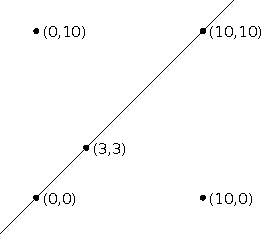
\includegraphics[width=0.30\textwidth]{sample1.pdf}}
  \hspace{0.20\textwidth}
  \subfigure[Sample input 2: No line with at least 3 points exists.]{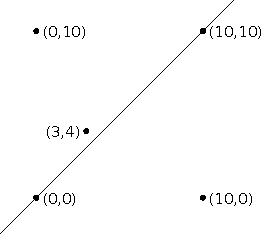
\includegraphics[width=0.30\textwidth]{sample2.pdf}}
  \caption{Illustration of the sample inputs}
\end{figure}
